\section{Discussion}

\subsection{Emulating System Dynamics}
Due to the continuous time-semantics which can be expressed in our agent-based approach we can also emulate SD. Every stock and flow is then just an agent which exchange messages where the simulation is stepped using the \textit{parallel} update-strategy. We add wrappers and type-definitions for convenience which increases the expressivity of the code, resembling system dynamics specifications. As a proof-of-concept we emulated the system dynamics of the SIR model, the code can be seen in Appendix \ref{app:sd_code}. Note that the code really looks like a SD specification with the integrals of the mathematical specification directly showing up in the code - the implementation is correct per definition. Due to the internal implementation of the \textit{integral} function of Yampa which uses the rectangle-rule to integrate, one must ensure to sample the system dynamics with small enough $\Delta t$ as becomes apparent in Figure \ref{fig:sd_plots}.

\begin{figure*}
\begin{center}
	\begin{tabular}{c c}
		\begin{subfigure}[b]{0.5\textwidth}
			\centering
			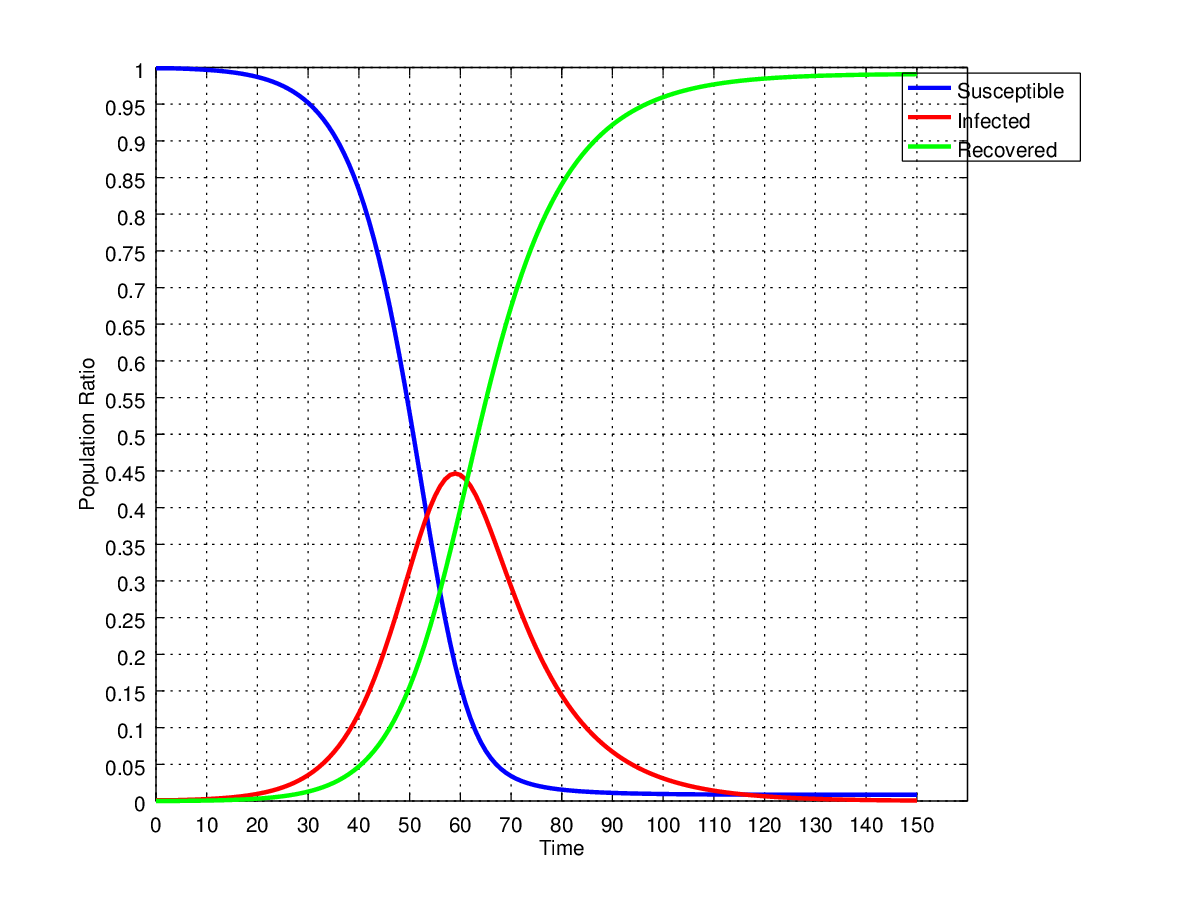
\includegraphics[width=.8\textwidth, angle=0]{./../shared/fig/frsd/SIR_SD_1000agents_150t_1dt.png}
			\caption{$\Delta t = 1.0$}
			\label{fig:sd_plot_10dt}
		\end{subfigure}
	
		& 
		
		\begin{subfigure}[b]{0.5\textwidth}
			\centering
			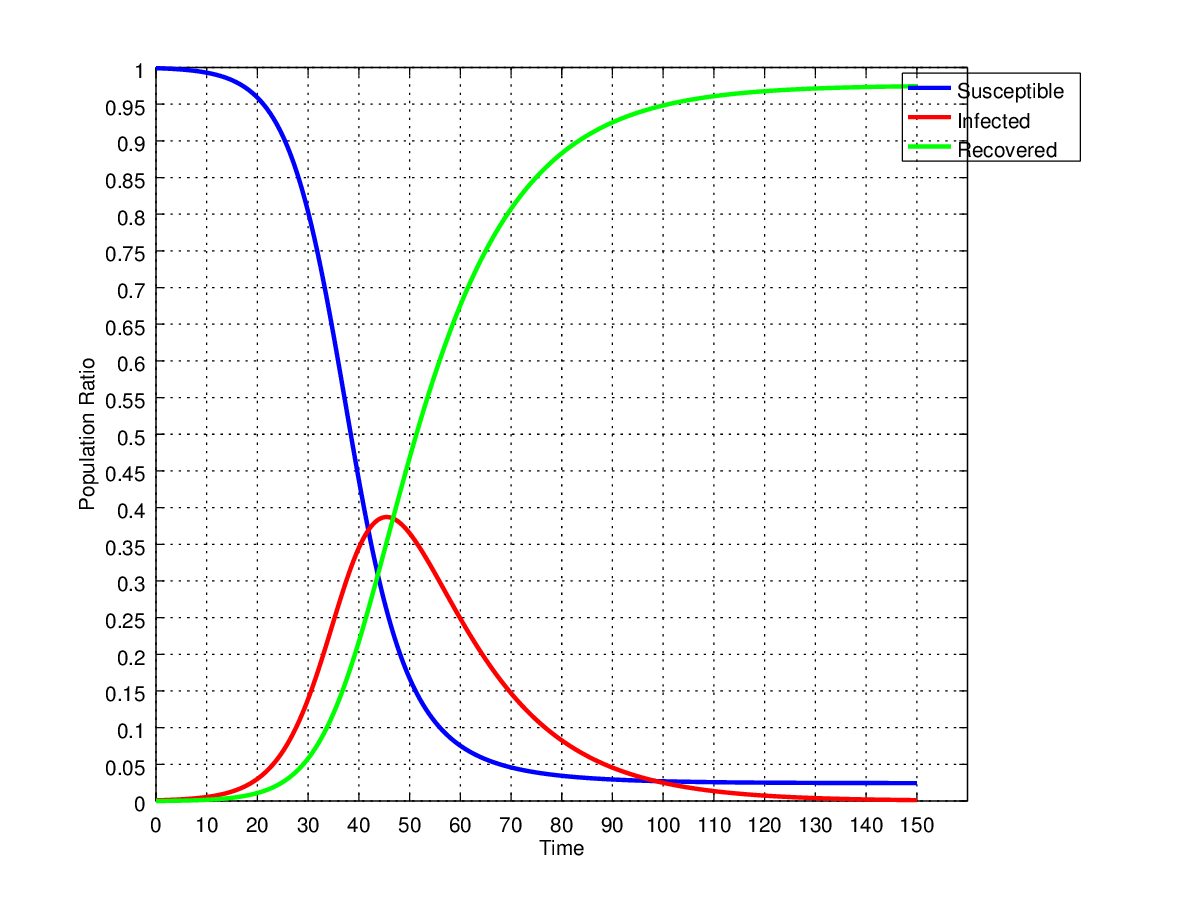
\includegraphics[width=.8\textwidth, angle=0]{./../shared/fig/frsd/SIR_SD_1000agents_150t_01dt.png}
			\caption{$\Delta t = 0.1$}
			\label{fig:sd_plot_0.1dt}
		\end{subfigure}
	\end{tabular}
	
	\caption{Simulating the SIR model with our SD emulation using different $\Delta t $. Note that although $\Delta t = 0.1$ might seem very close the system dynamic solution, there are still subtle differences to the initial Figure \ref{fig:sir_sd_dynamics} which uses $\Delta t = 0.01$.}
	\label{fig:sd_plots}
\end{center}
\end{figure*}

\subsection{Recursive ABS}
Due to the inherent recursive nature of functional programming we came up with the idea of \textit{recursive} ABS in which agents can recursively run the simulation within the simulation which would allow them to project their own actions into the future. So far it only exists as a proof-of-concept and we are currently only aware of a single model \cite{gilmer_recursive_2000} in the field of ABS which does recursive simulation. The implementation of recursive ABS is very natural due to the explicit data-flow and lack of side-effects which eases the task very much. Unfortunately we cannot go into detail of our approach as it is beyond the scope of the paper.


\subsection{Different Agent-Types}
[ ] can we implement different types of agents interacting with each other in the same simulation ? with different behaviour funcs, digferent state? yes, also not possible in NetLogo to my knowledge. but they must have the same messages, emvironment 

\subsection{Advantages}
	- no side-effects within agents leads to much safer code
	- edsl for time-semantics
	- declarative style: agent-implementation looks like a model-specification
	- reasoning and verification
	- sequential and parallel
	- powerful time-semantics
	- arrowized programming is optional and only required when utilizing yampas time-semantics. if the model does not rely on time-semantics, it can use monadic-programming by building on the existing monadic functions in the EDSL which allow to run in the State-Monad which simplifies things very much
	- when to use yampas arrowized programing: time-semantics, simple state-chart agents 
	- when not using yampas facilities: in all the other cases e.g. SugarScape is such a case as it proceeds in unit time-steps and all agents act in every time-step
	- can implement System Dynamics building on Yampas facilities with total ease	
	- get replications for free without having to worry about side-effects and can even run them in parallel without headaches
	- cant mess around with time because delta-time is hidden from you (intentional design-decision by Yampa). this would be only very difficult and cumbersome to achieve in an object-oriented approach. TODO: experiment with it in Java - how could we actually implement this? I think it is impossible: may only achieve this through complicated application of patterns and inheritance but then has the problem of how to update the dt and more important how to deal with functions like integral which accumulates a value through closures and continuations. We could do this in OO by having a general base-class e.g. ContinuousTime which provides functions like updateDt and integrate, but we could only accumulate a single integral value.
	- reproducibility statically guaranteed
	- cannot mess around with dt
	- code == specification
	- rule out serious class of bugs
	- different time-sampling leads to different results e.g. in wildfire \& SIR but not in Prisoners Dilemma. why? probabilistic time-sampling?
	- reasoning about equivalence between SD and ABS implementation in the same framework
	- recursive implementations
	
	- we can statically guarantee the reproducibility of the simulation because: no side effects possible within the agents which would result in differences between same runs (e.g. file access, networking, threading), also timedeltas are fixed and do not depend on rendering performance or userinput	
	
\subsection{Disadvantages}
	- performance is low
	- reasoning about performance is very difficult
	- very steep learning curve for non-functional programmers
	- learning a new EDSL
	- think ABMS different: when to use async messages, when to use sync conversations


[ ] important: increasing sampling freqzency and increasing number of steps so that the same number of simulation steps are executed should lead to same results. but it doesnt. why?
[ ] hypothesis: if time-semantics are involved then event ordering becomes relevant for emergent patterns. there are no tine semantics in heroes and cowards but in the prisoners dilemma
[ ] can we implement different types of agents interacting with each other in the same simulation ? with different behaviour funcs, digferent state? yes, also not possible in NetLogo to my knowledge. but they must have the same messages, emvironment 

[ ] Hypothesis: we can combine with FrABS agent-based simulation and system dynamics